\section{Architecture of the Controller Layer}

\subsection{Overview in the ROS2 Context}

As shown in the \textbf{Figure 1}, the ROS2 flow  starts with a high level node (User or just a normal Node) that sends a high level command to a 
\textbf{3rd party ros2 library} \textbf{(Moveit2)} which is responsible for the motion planning.
The 3rd party library sends the planned trajectory the \textbf{ROS2-controller} layer which contains a \textbf{controller management layer} and a \textbf{ Resource management layer}.
The planned trajectory entries the \textbf{controller management layer} which communicates with the \textbf{hardware} through the \textbf{ Resource management layer}.
The \textbf{ Resource management layer} contains user defined interfaces to communicate with the \textbf{hardware or the simulation}.\cite{ros2controllersoverview}


\begin{figure}[h]
    \centering
    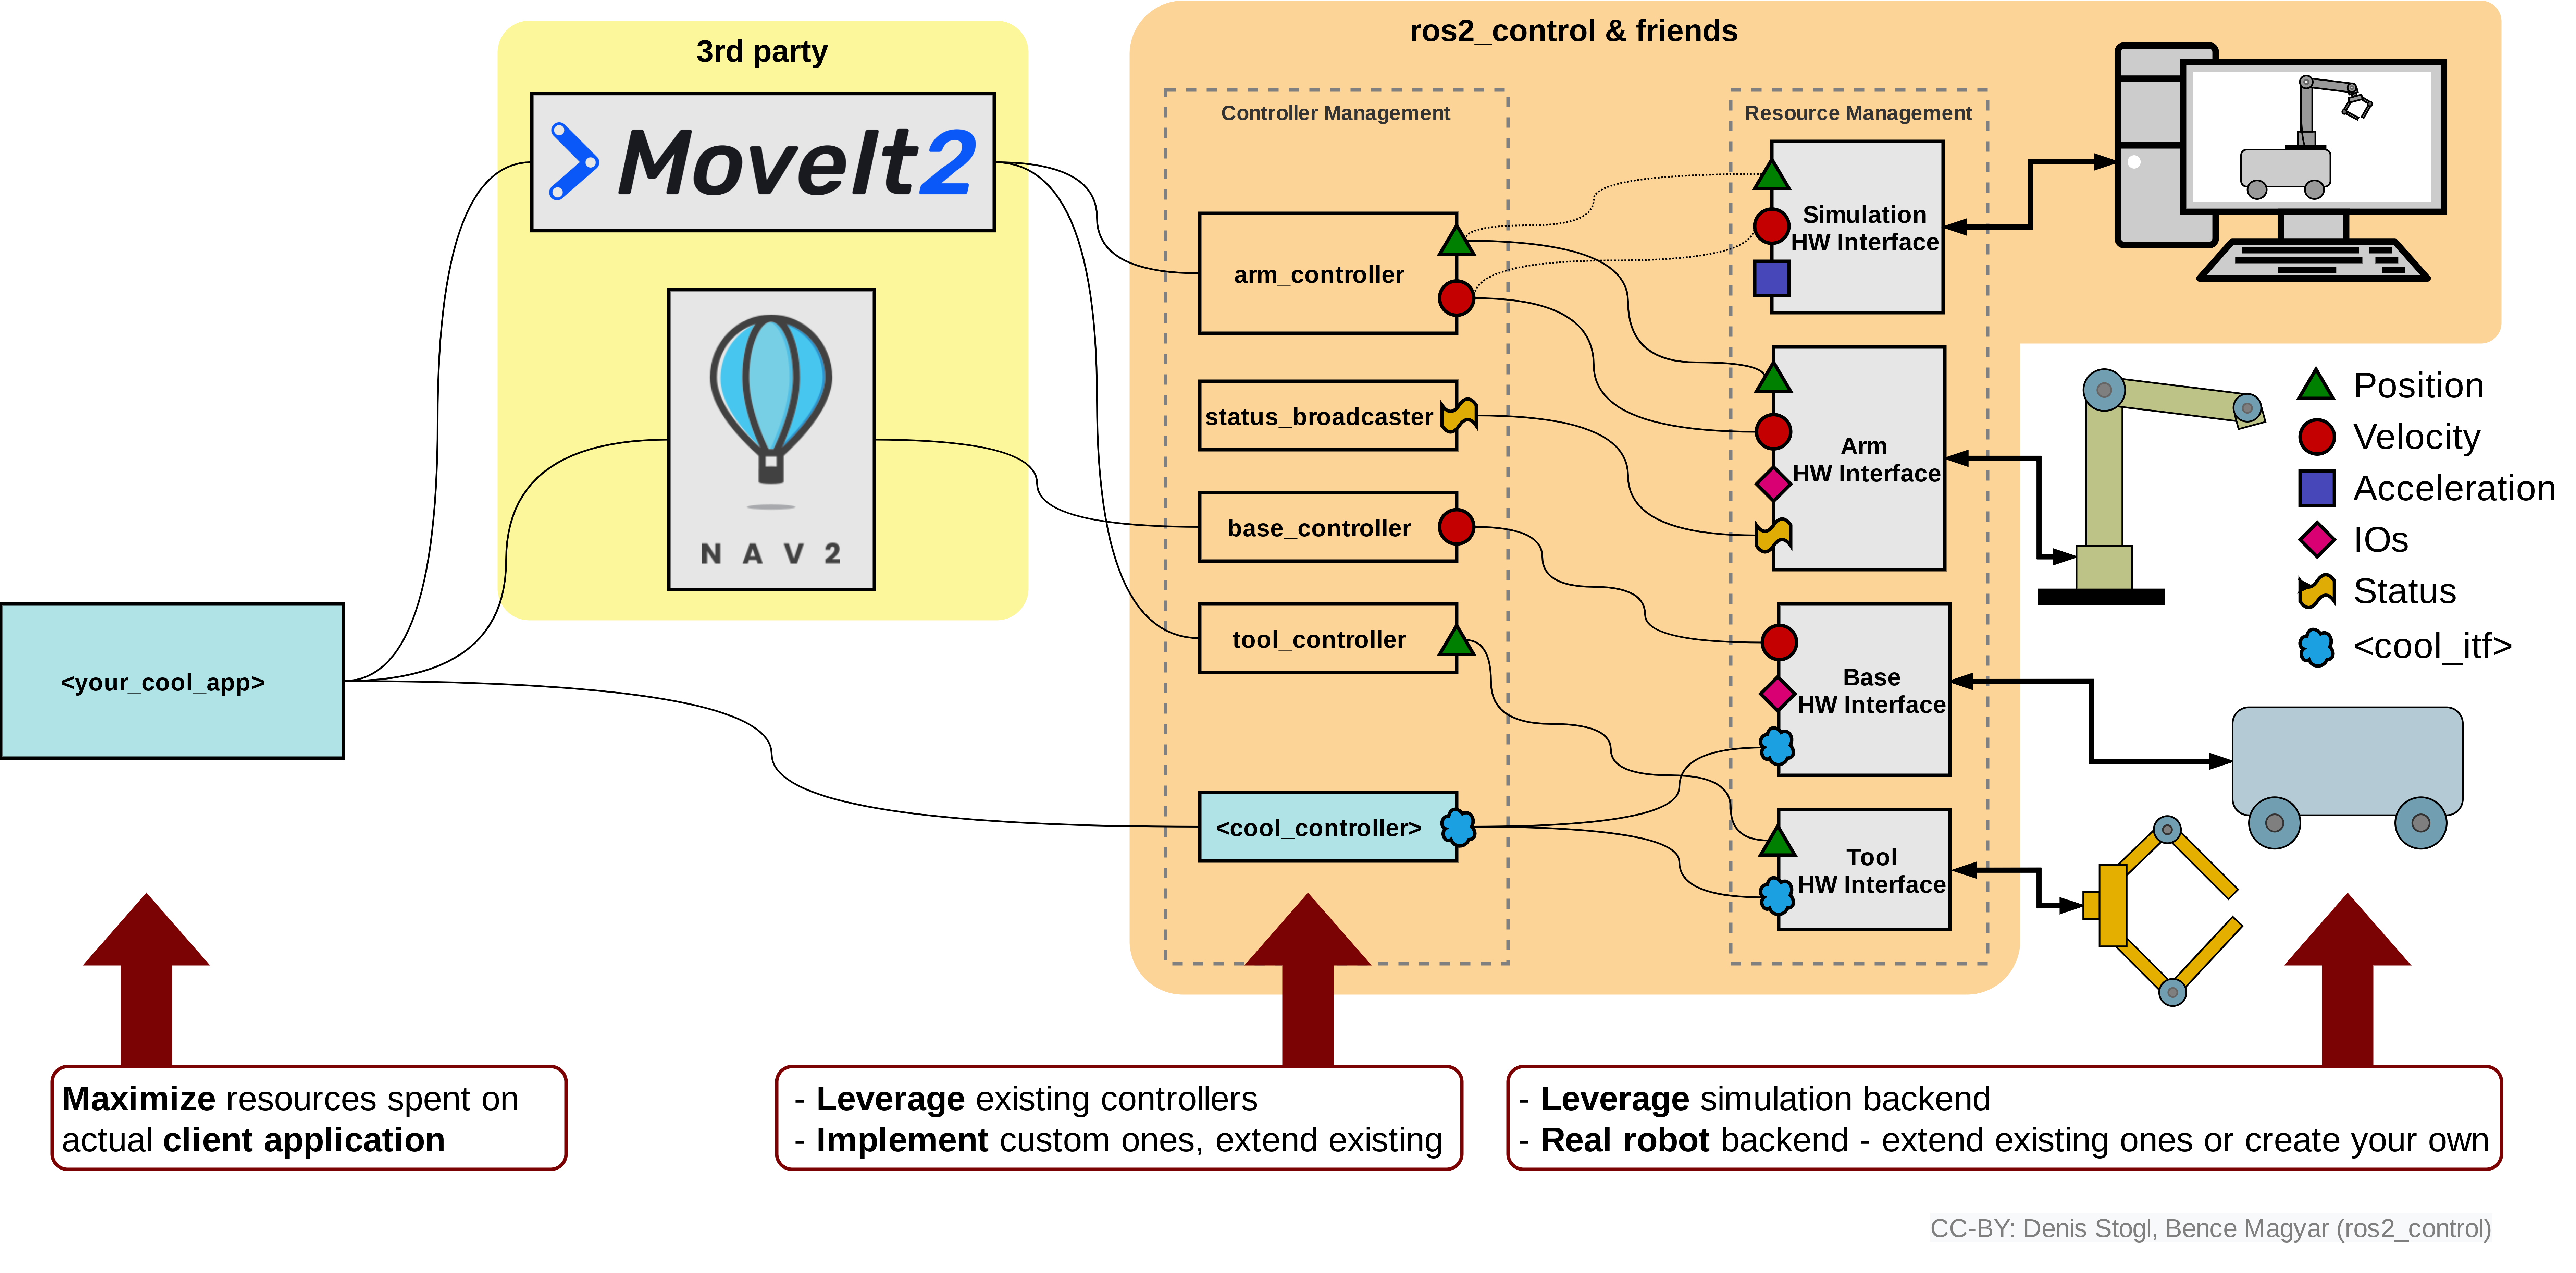
\includegraphics[width=0.9\textwidth]{ros2_controll_concept.png}
    \caption{ROS2 control Concept}
    \label{fig:mesh2}
\end{figure}

\newpage

\subsection{ROS2-controller Components}

the \textbf{Figure 2} is describing the main components of the ROS2 controller , the is a set of controllers 
"A, B, C", these controllers are mainly a yaml file with parameters that are passed to the controller manager.
On the other side the Resource manager collects all the hardware interfaces as plugins libraries and connects them to the controller manager.
Also the hardware interfaces are mainly two types , a command interface where the controller manager reads and writes to it and a state interface where the controller manager reads from it.\cite{ros2controllersarch}

\begin{figure}[h]
    \centering
    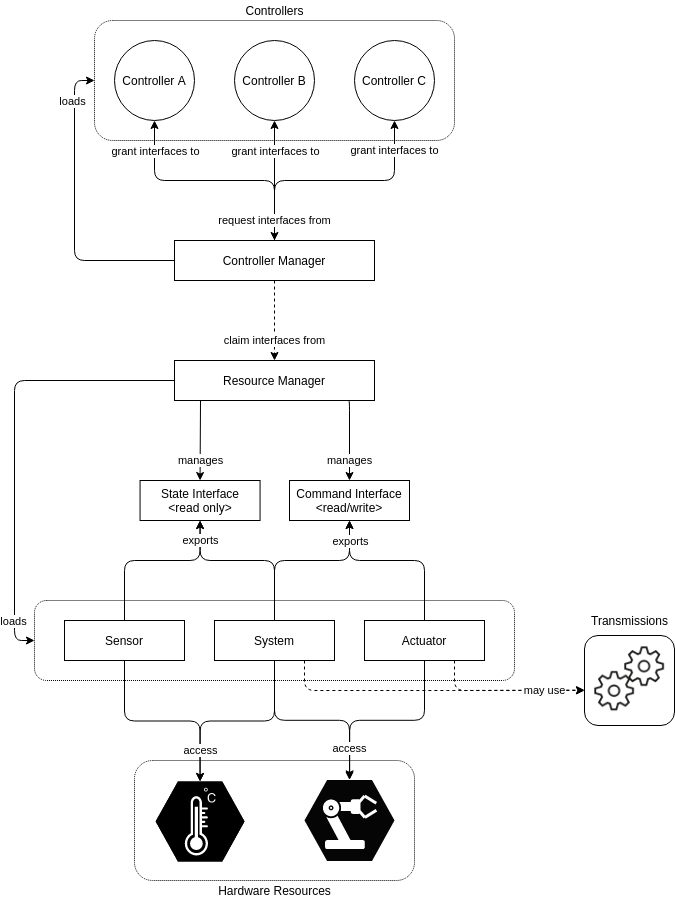
\includegraphics[width=0.7\textwidth]{components_architecture.png}
    \caption{ROS2 control components}
    \label{fig:mesh3}
\end{figure}
